\section[Olaf's Farm]{
    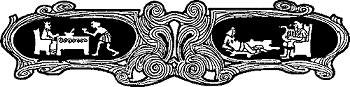
\includegraphics[width=9.3cm]{viking-tales/015}\\
    Olaf's Farm}

\lettrine{A}{t} another time Harald asked:
\vskip2\baselineskip
``What is your country, Olaf? Have you always been a thrall?''

The thrall's eyes flashed.

``When you are a man,'' he said, ``and go a-viking to Denmark, ask men
whether they ever heard of Olaf the Crafty. There, far off, is my
country, across the water. My father was Gudbrand the Big. Two hundred
warriors feasted in his hall and followed him to battle. Ten sons sat at
meat with him, and I was the youngest. One day he said:

```You are all grown to be men. There is not elbow-room here for so many
chiefs. The eldest of you shall have my farm when I die. The rest of
you, off a-viking!'

``He had three ships. These he gave to three of my brothers. But I stayed
that spring and built me a boat. I made her for only twenty oars because
I thought few men would follow me; for I was young, fifteen years old. I
made her in the likeness of a dragon. At the prow I carved the head with
open mouth and forked tongue thrust out. I painted the eyes red for
anger.

```There, stand so!' I said, `and glare and hiss at my foes.'

``In the stern I curved the tail up almost as high as the head. There I
put the pilot's seat and a strong tiller for the rudder. On the breast
and sides I carved the dragon's scales. Then I painted it all black and
on the tip of every scale I put gold. I called her `Waverunner.' There
she sat on the rollers, as fair a ship as I ever saw.

``The night that it was finished I went to my father's feast. After the
meats were eaten and the mead-horns came round, I stood up from my bench
and raised my drinking-horn\footnote{See note about drinking-horns on
page~\pageref{drinking-horns}.} high and spoke with a great voice:

```This is my vow: I will sail to Norway and I will harry the coast and
fill my boat with riches. Then I will get me a farm and will winter in
that land. Now who will follow me?'

```He is but a boy,' the men said. `He has opened his mouth wider than he
can do.'

``But others jumped to their feet with their mead-horns in their hands.
Thirty men, one after another, raised their horns and said:

```I will follow this lad, and I will not turn back so long as he and I
live!'

``On the next morning we got into my dragon and started. I sat high in
the pilot's seat. As our boat flashed down the rollers into the water I
made this song and sang it:

\begin{quote}
```The dragon runs.\\
Where will she steer?\\
Where swords will sing,\\
Where spears will bite,\\
Where I shall laugh.'
\end{quote}

``So we harried the coast of Norway. We ate at many men's tables
uninvited. Many men we found overburdened with gold. Then I said:

```My dragon's belly is never full,' and on board went the gold.

``Oh! it is better to live on the sea and let other men raise your crops
and cook your meals. A house smells of smoke, a ship smells of frolic.
From a house you see a sooty roof, from a ship you see Valhalla.

``Up and down the water we went to get much wealth and much frolic. After
a while my men said:

```What of the farm, Olaf?'

```Not yet,' I answered. `Viking is better for summer. When the ice
comes, and our dragon cannot play, then we will get our farm and sit
down.'

``At last the winter came, and I said to my men:

```Now for the farm. I have my eye on one up the coast a way in King
Halfdan's country.'

``So we set off for it. We landed late at night and pulled our boat up on
shore and walked quietly to the house. It was rather a wealthy farm, for
there were stables and a storehouse and a smithy at the sides of the
house. There was but one door to the house. We went to it, and I struck
it with my spear.

\begin{figure}
    \centering
    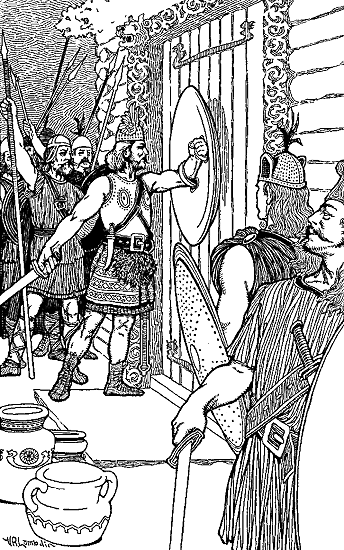
\includegraphics[width=9.1cm]{viking-tales/016}
    \caption{
        ``I struck my shield against the door so that it made a great
        clanging''}
\end{figure}

```Hello! Ho! Hello!' I shouted, and my men made a great din.

``At last some one from inside said:

```Who calls?'

```I call,' I answered. `Open! or you will think it Thor who calls,' and
I struck my shield against the door so that it made a great clanging.

``The door opened only a little, but I pushed it wide and leaped into the
room. It was so dark that I could see nothing but a few sparks on the
hearth. I stood with my back to the wall; for I wanted no sword reaching
out of the dark for me.

```Now start up the fire,' I said.

```Come, come!' I called, when no one obeyed. `A fire! This is cold
welcome for your guests.'

``My men laughed.

```Yes, a stingy host! He acts as though he had not expected us.'

``But now the farmer was blowing on the coals and putting on fresh wood.
Soon it blazed up, and we could see about us. We were in a little feast
hall,\footnote{See note about feast hall on page~\pageref{feast-hall}.}
with its fire down the middle of it. There were benches for twenty men
along each side. The farmer crouched by the fire, afraid to move. On a
bench in a far corner were a dozen people huddled together.

```Ho, thralls!' I called to them. `Bring in the table. We are hungry.'

``Off they ran through a door at the back of the hall. My men came in and
lay down by the fire and warmed themselves, but I set two of them as
guards at the door.

```Well, friend farmer,' laughed one, `why such a long face? Do you not
think we shall be merry company?'

```We came only to cheer you,' said another. `What man wants to spend the
winter with no guests?'

```Ah!' another then cried out, sitting up. `Here comes something that
will be a welcome guest to my stomach.'

``The thralls were bringing in a great pot of meat. They set up a crane
over the fire and hung the pot upon it, and we sat and watched it boil
while we joked. At last the supper began. The farmer sat gloomily on the
bench and would not eat, and you cannot wonder; for he saw us putting
potfuls of his good beef and basket-loads of bread into our big mouths.
When the tables were taken out and the mead-horns came round, I stood up
and raised my horn and said to the farmer:

```You would not eat with us. You cannot say no to half of my ale. I
drink this to your health.'

``Then I drank half of the hornful and sent the rest across the fire to
the farmer. He took it and smiled, saying:

```Since it is to my health, I will drink it. I thought that all this
night's work would be my death.'

```Oh, do not fear that!' I laughed, `for a dead man sets no tables.'

``So we drank and all grew merrier. At last I stood up and said:

```I like this little taste of your hospitality, friend farmer. I have
decided to accept more of it.'

``My men roared with laughter.

```Come,' they cried, `thank him for that, farmer. Did you ever have such
a lordly guest before?'

``I went on:

```Now there is no fun in having guests unless they keep you company and
make you merry. So I will give out this law: that my men shall never
leave you alone. Hakon there shall be your constant companion, friend
farmer. He shall not leave you day or night, whether you are working or
playing or sleeping. Leif and Grim shall be the same kind of friends to
your two sons.'

``I named nine others and said:

```And these shall follow your thralls in the same way. Now, am I not
careful to make your time go merrily?'

``So I set guards over every one in that house. Not once all that winter
did they stir out of sight of some of us. So no tales got out to the
neighbors. Besides, it was a lonely place, and by good luck no one came
that way. Oh! that was fat and easy living.

``Well, after we had been there for a long time, Hakon came in to the
feast one night and said:

```I heard a cuckoo to-day!'

```It is the call to go a-viking,' I said.

``All my men put their hands to their mouths and shouted. Their eyes
danced. Big Thorleif stood up and stretched himself.

```I am stiff with long sitting,' he said. `I itch for a fight.'

``I turned to the farmer.

```This is our last feast with you,' I said.

```Well,' he laughed, `this has been the busiest winter I ever spent, and
the merriest. May good luck go with you!'

```By the beard of Odin!' I cried; `you have taken our joke like a man.'

``My men pounded the table with their fists.

```By the hammer of Thor!' shouted Grim. `Here is no stingy coward. He is
a man fit to carry my drinking-horn, the horn of a sea-rover and a
sword-swinger. Here, friend, take it,' and he thrust it into the
farmer's hand. `May you drink heart's-ease from it for many years. And
with it I leave you a name, Sif the Friendly. I shall hope to drink with
you sometime in Valhalla.'

``Then all my men poured around that farmer and clapped him on the
shoulder and piled things upon him, saying:

```Here is a ring for Sif the Friendly.'

```And here is a bracelet.'

```A sword would not be ashamed to hang at your side.'

``I took five great bracelets of gold from our treasure chest and gave
them to him.

``The old man's eyes opened wide at all these things, and at the same
time he laughed.

```May Odin send me such guests every winter!' he said.

``Early next morning we shook hands with our host and boarded the
`Waverunner' and sailed off.

```Where shall we go?' my men asked.

```Let the gods decide,' I said, and tossed up my spear.

``When it fell on the deck it pointed up-shore, so I steered in that
direction. That is the best way to decide, for the spear will always
point somewhere, and one thing is as good as another. That time it
pointed us into your father's ships. They closed in battle with us and
killed my men and sunk my ship and dragged me off a prisoner. They were
three against one, or they might have tasted something more bitter at
our hands. They took me before King Halfdan.

```Here,' they said, `is a rascal who has been harrying our coasts. We
sunk his ship and men, but him we brought to you.'

```A robber viking?' said the king, and scowled at me.

``I threw back my head and laughed.

```Yes. And with all your fingers it took you a year to catch me.'

``The king frowned more angrily.

```Saucy, too?' he said. `Well, thieves must die. Take him out, Thorkel,
and let him taste your sword.'

``Your mother, the queen, was standing by. Now she put her hand on his
arm and smiled and said:

```He is only a lad. Let him live. And would he not be a good gift for
our baby?'

``Your father thought a moment, then looked at your mother and smiled.

```Soft heart!' he said gently to her; then to Thorkel, `Well, let him
go, Thorkel!'

``Then he turned to me again, frowning.

```But, young sharp-tongue, now that we have caught you we will put you
into a trap that you cannot get out of. Weld an iron collar on his
neck.'

``So I lived and now am your tooth thrall. Well, it is the luck of war.
But by the chair of Odin, I kept my vow!''

``Yes!'' cried Harald, jumping to his feet. ``And had a joke into the
bargain. Ah! sometime I will make a brave vow like that.''

\begin{figure}[hb]
    \centering
    \vskip8pt
    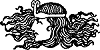
\includegraphics[width=2.7cm]{viking-tales/017}
\end{figure}
